\documentclass[a4paper, 12pt]{article}
\usepackage[utf8]{inputenc}
\usepackage[english, ukrainian]{babel}
\usepackage{amsmath, amssymb}
\usepackage[top = 2 cm, left = 1 cm, right = 1 cm, bottom = 2 cm]{geometry} 

\usepackage{float}
\usepackage{hyperref}
\usepackage{verbatim}
\usepackage{graphicx}

\setlength{\parindent}{0 cm}

\title{Аналіз даних за допомогою пакету R}
\author{Нікіта Скибицький}
\date{\today}

\begin{document}

\maketitle

\thispagestyle{empty}

\newpage

\section{Початок роботи з системою R}

Завантажте R (для Windows) за \href{https://cloud.r-project.org/bin/windows/base/}{посиланням} (станом на \today остання версія 3.5.1) та встановіть його. \\

Завантажте RStudio (для Windows) за \href{https://download1.rstudio.org/RStudio-1.1.463.exe}{посиланням} (станом на \today остання версія 1.1.463) та встановіть її. \\

Запустіть RStudio (наприклад виконавши \verb|start rstudio.exe| у командному рядку). Ви побачите приблизно наступний еркан (швидше за все із світлою темою):
\begin{figure}[H]
	\centering
	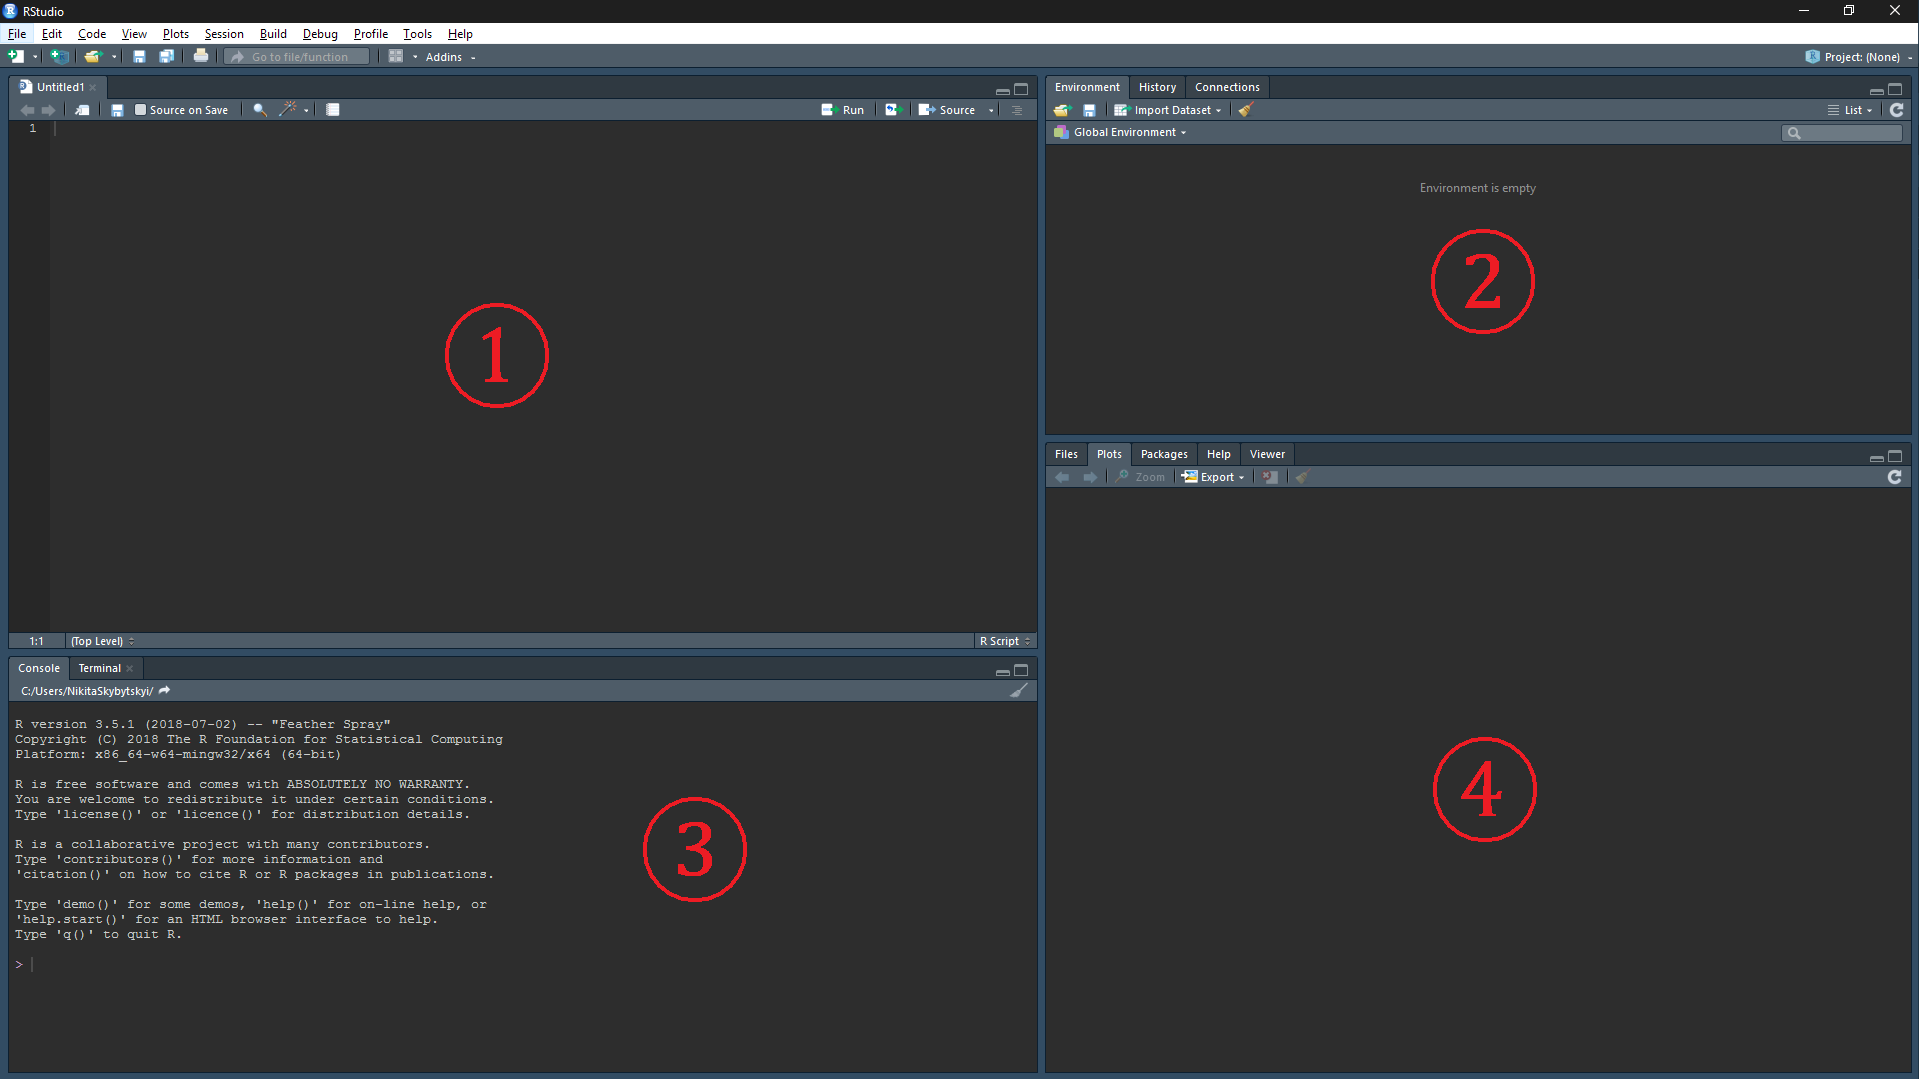
\includegraphics[width=\linewidth]{rstudio-workplace-1-2-3-4.png}
\end{figure}

Як бачимо, у нього є 4 основні частини:
\begin{enumerate}
	\item Текстовий редактор, у ньому ви набиратимете код.%:
	% \begin{figure}[H]
	% 	\centering
	% 	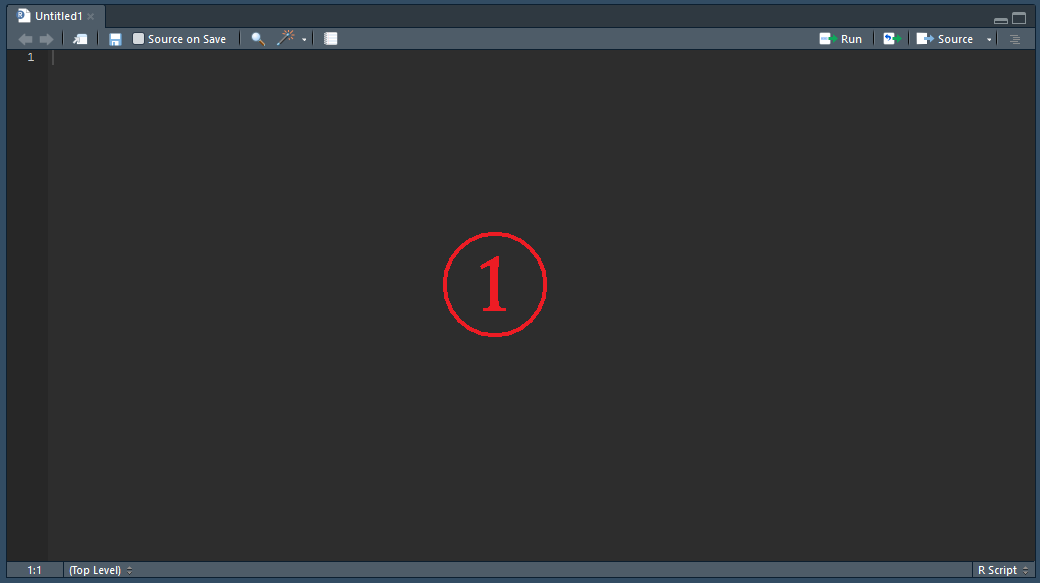
\includegraphics[width=.5\linewidth]{rstudio-workplace-1.png}
	% \end{figure}

	\item Інспектор середовища, через нього можна подивитися які імена визначені у середовищі виконання програми на даний момент і які значення їм відповідають.%:
	% \begin{figure}[H]
	% 	\centering
	% 	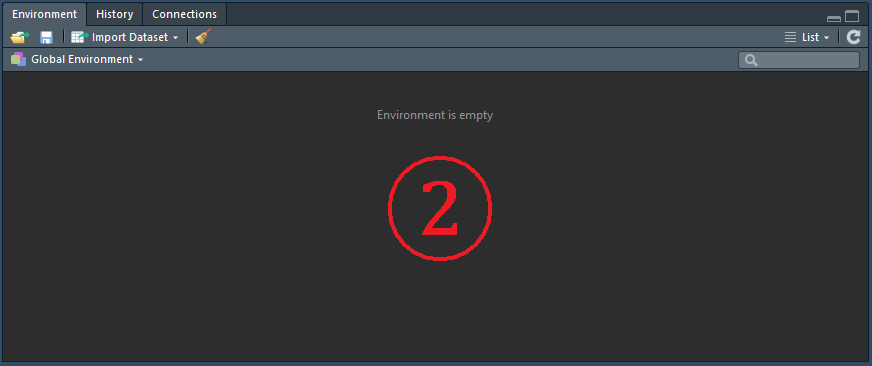
\includegraphics[width=.5\linewidth]{rstudio-workplace-2.png}
	% \end{figure}

	\item R-консоль і термінал, у них відображатимуться результати виконання R- та bash-команд відповідно.%:
	% \begin{figure}[H]
	% 	\centering
	% 	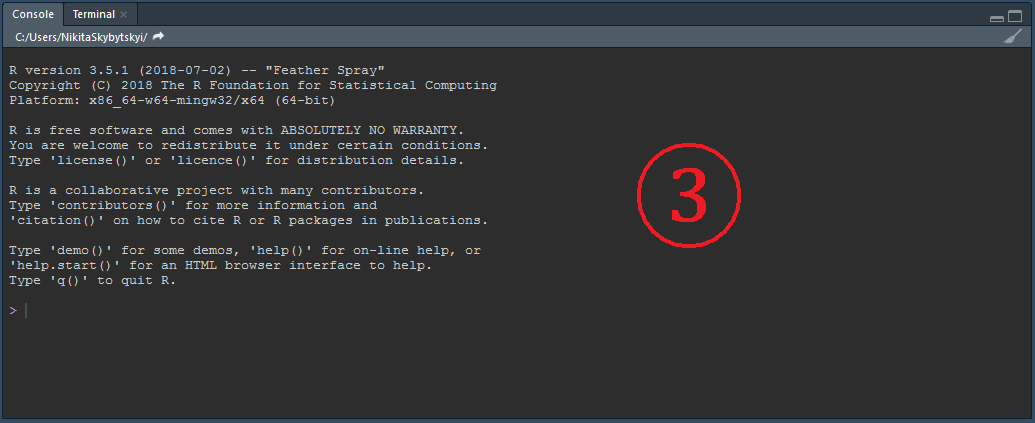
\includegraphics[width=.5\linewidth]{rstudio-workplace-3.png}
	% \end{figure}

	\item Інспектор графіків, у ньому відображатимуться усі графіки які ви малюватимете.%:
	% \begin{figure}[H]
	% 	\centering
	% 	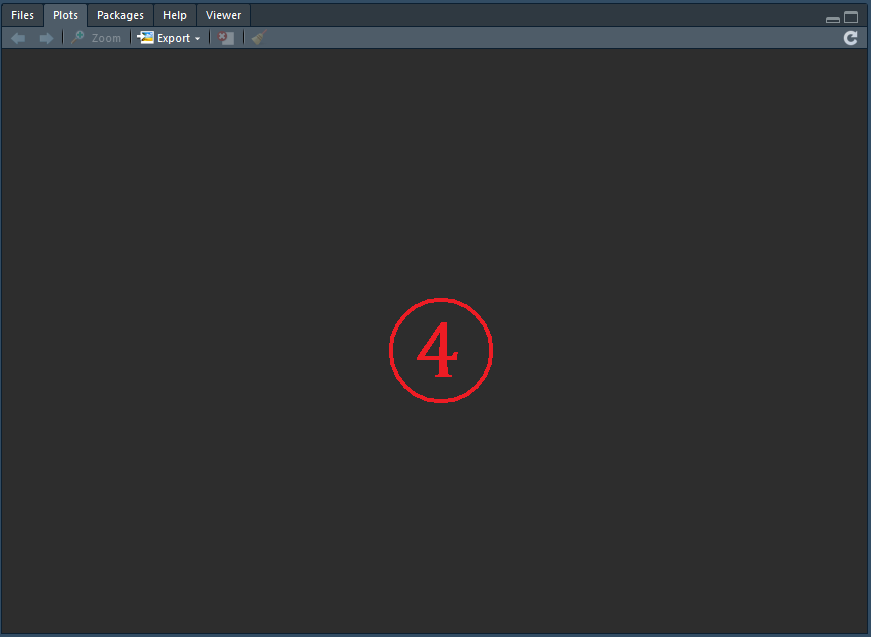
\includegraphics[width=.5\linewidth]{rstudio-workplace-4.png}
	% \end{figure}
\end{enumerate}

Для початку можете погратися із R як із калькулятором, вводячи у R-консоль (третя область на малюнках вище) арифметчині вирази і спостерігаючи результат їх обчислення:
\begin{verbatim}
> 1 + 2
[1] 3
> 3 - 4
[1] -1
> 4 * 5
[1] 20
> 6 / 7
[1] 0.8571429
> 8^9
[1] 134217728
\end{verbatim}

Виконати поточну команду у консолі можна клавішею \verb|Return| (також відома як \verb|Enter|), а у текстовому редакторі -- комбінацією клавіш \verb|Ctrl+Return|. (Командою вважається рядок на якому знаходиться курсор, або виділена частина скрипта якщо така є). \\

Як і у мові програмування \verb|python|, більшість функціональності не вбудована в мову програмування, а реалізована у R-пакетах (англ. R-packages). Підключити встановлений пакет можна за допомогою функції \verb|library()|, а встановити новий пакет -- функцією \verb|install.packages()|.

\begin{verbatim}
> library(splines)  # підключаємо встановлений за замовчуванням пакет

> library(abctools)  # намагаємося підключити не встановлений пакет і ловимо помилку:
Error in library(abctools) : there is no package called ‘abctools’

> install.packages("abctools")  # встановлюємо пакет, разом зі всіма його залежностями:
Installing package into ‘C:/Users/NikitaSkybytskyi/Documents/R/win-library/3.5’
(as ‘lib’ is unspecified)
also installing the dependencies ‘SparseM’, ..., ‘Hmisc’

trying URL 'https://cran.rstudio.com/bin/windows/contrib/3.5/SparseM_1.77.zip'
Content type 'application/zip' length 1374637 bytes (1.3 MB)
downloaded 1.3 MB

...

trying URL 'https://cran.rstudio.com/bin/windows/contrib/3.5/Hmisc_4.1-1.zip'
Content type 'application/zip' length 3013429 bytes (2.9 MB)
downloaded 2.9 MB

trying URL 'https://cran.rstudio.com/bin/windows/contrib/3.5/abctools_1.1.3.zip'
Content type 'application/zip' length 2803903 bytes (2.7 MB)
downloaded 2.7 MB

package ‘SparseM’ successfully unpacked and MD5 sums checked
...
package ‘Hmisc’ successfully unpacked and MD5 sums checked
package ‘abctools’ successfully unpacked and MD5 sums checked

The downloaded binary packages are in
	C:\Users\NikitaSkybytskyi\AppData\Local\Temp\RtmpUNppEz\downloaded_packages

> library(abctools)  # успішно підключаємо щойно встановлений пакет:
Loading required package: abc
...
abctools 1.1.3 loaded
\end{verbatim}

З цікавих особливостей зауважимо ще, що R може зберігати образ середеовища, що дозволяє продовжувати роботу з того з місця на якому ви зупинилися минулого разу без необхідності заново визначати значення всіх визначених імен. Якщо це саме те що вам потрібно, то у діалозі при закритті RStudio виберіть ``зберегти образ робочого середовища'':
\begin{figure}[H]
	\centering
	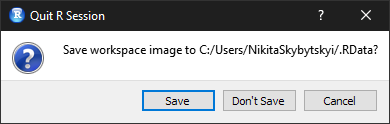
\includegraphics[width=.5\linewidth]{quit-r-session.png}
\end{figure}

У мові програмування S (так, R не є мовою програмування, а радше просто інтерпретатором), як і будь-якій іншій потужній мові легко загубитися початківцю. Як завжди, рекомендуємо звертатися до офіційної документації окремих пакетів, і знаходити відповіді на свої запитання (котрих майже напевно буде не мало) на теренах \href{https://stackoverflow.com}{stackoverflow}.

\section{Робота з даними (найпростіші операції і типи даних)}

\subsection{Арифметичні операції в R}

Позначаються, як ми вже бачили вище, звичайним чином: \verb|+|, \verb|-|, \verb|*|, \verb|/| і \verb|^| для піднесення до степеню. Порядок виконання операцій звичайний і може бути змінений за допомогою дужок:
\begin{verbatim}
> 7 * (3 + 12) / 2 - 7^2
[1] 3.5
\end{verbatim}

Також є в наявності елементарні функції: \verb|log()|, \verb|log10()|, \verb|exp()|, \verb|sin()|, \verb|cos()|, \verb|tan()|, \verb|sqrt()|, а також \verb|abs()|. Функція \verb|round(x, n)| округлює число \verb|x| до \verb|n| десяткових знаків після коми.

\subsection{Логічні операції}

Це операції: \verb|<|, \verb|>|, \verb|<=| (менше або дорівнює); \verb|>=| (більше або дорівнює); \verb|==| (дорівнює); \verb|!=| (не дорівнює); \verb| &| (логічне ``і''); \tt|\normalfont (логічне ``або'').

\subsection{Присвоєння значення імені} 
Традиційно здійснюється за допомогою символу \verb|<-|. Також використовується знак \verb|=|:
\begin{verbatim}
> x <- 7
> x + 3
[1] 10
\end{verbatim}

\subsection{Статистичні операції}
\begin{itemize}
	\item \verb|mean(x)| обчислює вибіркове середнє масиву \verb|х|;

	\item \verb|sd(x)| обчислює вибіркове середньоквадратичне відхилення \verb|х|;

	\item \verb|var(x)| обчислює вибіркову дисперсію масиву \verb|х|;

	\item \verb|summary(x)| виводить елементи дескриптивної статистики масиву \verb|х|: мінімальне значення, максимальне, обидва квартилі, медіану і середнє.

	\item \verb|range(x)| повертає найбільше і найменше значення в \verb|х|. Якщо нас цікавить різниця між найбільшим і найменшим значеннями, можна скористатись функцією \verb|diff(range(x))|. 

	\begin{verbatim}
	> range(1:10)  # 1:10 - послідовність цілих чисел від 1 до 10
	[1] 1 10
	> diff(range(1:10))
	[1] 9
	\end{verbatim}

	\item \verb|cor(x, y)| обчислює коефіцієнт кореляції Пірсона між масивами \verb|x| i \verb|y| однакової довжини. Якщо \verb|х| -- матриця, то команда \verb|cor(x, х)| видає матрицю кореляцій даних.

	\item Для обчислення коефіцієнта кореляції Спірмена необхідно в тій самій команді задати додатковий параметр \verb|method|:
	\begin{verbatim}
	> x <- c(-100, 0, 11)  # c() створює вектор із своїх аргументів
	> y <- c(134, 2, -6)
	> cor(x, y)
	[1] -0.9992336
	> cor(x, y, method = "spearman")
	[1] -1
	\end{verbatim}
\end{itemize}

\subsection{Вектори}

Створюємо вектор за допомогою функції \verb|c()|:
\begin{verbatim}
> x <- c(1.5, 2, 3)
> x
[1] 1.5 2.0 3.0
\end{verbatim}

У вектор можна помістити дані інших типів. Наприклад, текстові:
\begin{verbatim}
> y <- c("A", "Hello", "world!")
> y
[1] "A" "Hello" "world!"
\end{verbatim}

Можна з’єднати 2 вектори в одну структуру з двох стовпчиків. Для цього використовують функцію \verb|cbind()|:
\begin{verbatim}
> x <- c(2, 3, 4, 1)
> y <- c(1, 1, 1, 10)
> cbind(x, y)
     x  y
[1,] 2  1
[2,] 3  1
[3,] 4  1
[4,] 1 10
\end{verbatim}

Об‘єднання двох рядків в одну структуру здійснюється за допомогою \verb|rbind()|:
\begin{verbatim}
> rbind(x, y)
  [,1] [,2] [,3] [,4]
x    2    3    4    1
y    1    1    1   10
\end{verbatim}

Операції додавання, різниці, множення векторів відбуваються поелементно. Якщо ж вектори, що, наприклад, додаються, мають різні довжини, то коротший вектор ``циклічно'' продовжується до розміру довгого, і після цього проводиться додавання поелементно, причому генерується застереження:

\begin{verbatim}
> x <- c(-100, 0, 1, 5, -9, 8, 4)
> y <- c(1, 2)
> y + x
[1] -99 2 2 7 -8 10 5
Warning message:
In y + x : longer object length is not a multiple of shorter object length
\end{verbatim}

\subsection{Послідовності}

Команда \verb|seq()| створює послідовність чисел. Її часто використовують при графічному аналізі. Три аргументи, які зазвичай використовують в команді: початкове значення, кінцеве і крок (приріст). Якщо ж приріст \verb|= 1|, то достатньо двох аргументів:

\begin{verbatim}
> seq(0, 1, 0.2)
[1] 0.0 0.2 0.4 0.6 0.8 1.0
> seq(0, 8)
[1] 0 1 2 3 4 5 6 7 8
\end{verbatim}

Для стислого запису послідовності цілих від \verb|0| до \verb|8| можна скористатись діапазоном:

\begin{verbatim}
> 0:8
[1] 0 1 2 3 4 5 6 7 8
\end{verbatim}

Для повторення в послідовності \verb|n| разів однакових чисел або символів використовують команду \verb|rep(a, n)|:

\begin{verbatim}
> rep(c(0, "x"), 3)
[1] "0" "x" "0" "x" "0" "x"
\end{verbatim}

Також можна регулювати довжину послідовності.

\begin{verbatim}
> rep(c(1, 2, 3), length = 10)
[1] 1 2 3 1 2 3 1 2 3 1
\end{verbatim}

Відмітимо, що пакет R (як і будь-яка мова програмування яка себе поважає) використовує круглі дужки \verb|( )| для аргументів функцій і квадратні \verb|[ ]| для того, щоб звернутись до конкретного елемента в послідовності, векторі, масиві, списку. Також R підтримує концепції зрізу (англ. slice), індексації по бітовій, індексній та логічній масках, а також від'ємні індекси для індексації (у якомусь сенсі) з кінця:

\begin{verbatim}
> t <- C(2, 3, -1, 77, 128, 3)
> t[2]  # другий елемент
[1] 3
> t[2:4]  # елементи з другого по четвертий, включно
[1] 3 -1 77
> t[c(1, 4, 6)]  # елементи з індексами 1, 4 і 6
[1] 2 77 3
> t[t < 0]  # всі від'ємні елементи
[1] -1
> t[abs(t) > 70]  # всі елементи, за модулем більші ніж 70
[1] 77 128
> t[-1]  # всі окрім першого
[1] 3 -1 77 128 3
\end{verbatim}

Зауважимо, що пакет R (на відміну від будь-якої мови програмування яка себе поважає) починає індексацію з \verb|1| а не з \verb|0|, тому будьте обачні. \\

Абсолютно аналогічно індексація працює над іншими типами даних, наприклад над матрицями.

\subsection{Списки}

Список -- це структура, тобто вектор, елементи якого можуть мати різні типи: числові, текстові і т.д. Елементом списку може бути інший список. Списки створюються за допомогою функції \verb|list()|:
\begin{verbatim}
> student <- list(name = "Alex", surname = "Koval", major = "Math", entry.year = 2015)
> student[[4]]  # індексація списків трохи відрізняється: [[]] замість []
[1] 2015
> student$entry.year  # також можливе пойменне звертання до полів списку
[1] 2015
\end{verbatim}

\subsection{Матриці}

\[ b = \begin{pmatrix}190  & 8  & 22.0 \\ 191  & 4  & 1.7 \\ 223  & 80  & 2.0\end{pmatrix}. \]

Створити таку матрицю в R можна за допомогою команди \verb|matrix()|. Присвоїмо їй ім’я \verb|b.data|. Якщо ми хочемо, щоб дані записувались в матрицю по рядках, використовуємо опцію \verb|byrow = TRUE|. В даному прикладі опція \verb|nrow = 3| показує кількість рядків матриці:
\begin{verbatim}
> Data <- c(190, 8, 22, 191, 4, 1.7, 223, 80, 2)
> b.data <- matrix(Data, nrow = 3, byrow = TRUE)
> b.data
     [,1] [,2]  [,3]
[1,]  190    8  22.0
[2,]  191    4   1.7
[3,]  223   80   2.0
> dim(b.data)  # розмірність матриці
[1] 3 3
> region <- c("East", "Middle", "West")  # імена розмірностей
> dimnames(b.data) <- list(region, NULL)
> b.data
       [,1] [,2]  [,3]
East    190    8  22.0
Middle  191    4   1.7
West    223   80   2.0
> type <- c("type A", "type B", "type C")  # імена розмірностей
> dimnames(b.data) <- list(NULL, type)
> b.data
     type A  type B  type C
[1,]    190       8    22.0
[2,]    191       4     1.7
[3,]    223      80     2.0
> dimnames(b.data) <- list(region, type)  # імена розмірностей
> b.data
       type A  type B  type C
East      190       8    22.0
Middle    191       4     1.7
West      223      80     2.0
\end{verbatim}
Додавання матриць \verb|А + В| відбувається поелементно. Множення \verb|А * В| також – поелементно. Якщо матриці мають різну розмірність, то операція не виконується. \\

Операція множення матриць в математичному сенсі виглядає як \verb|A %*% B|:
\begin{verbatim}
> Data <- c(1, 0, 0, 1)
> A <- matrix(Data, nrow = 2, byrow = TRUE)
> A
     [,1] [,2]
[1,]    1    0
[2,]    0    1
> Data <- c(1, -9, 1, 1)
> B <- matrix(Data, nrow = 2, byrow = TRUE)
> C <- A %*% B
> C
     [,1] [,2]
[1,]    1   -9
[2,]    1    1
\end{verbatim}

Операція \verb|diag()| перетворює діагональні елементи матриці в елементи вектора:
\begin{verbatim}
> z <- diag(C)
> z
[1] 1 1
\end{verbatim}

\subsection{Фрейми даних}

Фрейм -- найбільш широковживаний тип змінних в R, який використовується для зберігання даних. Фрейми складаються з різноманітних типів даних (числових, текстових, логічних і т.д.). Традиційно, стовпчики розглядаються як змінні, рядки містять характеристики об’єктів. Приклад:

\begin{enumerate}
\item Створюємо файл \verb|*.txt| з даними. Зчитуємо ці дані у фрейм за допомогою команди

\begin{verbatim}
> da <- read.table(file.choose(), header = TRUE)
> da
       Value_A  Value_B  Value_C
First      190        8     22.0
Second     191        4      1.7
Third      223       80      2.0
\end{verbatim}

\item Тепер ми хочемо залучити дві додаткові змінні: логічну змінну \verb|Opinion| і текстову \verb|Danger|. Створюємо відповідні стовпчики-масиви і заносимо їх у фрейм:

\begin{verbatim}
> Opinion <- c(FALSE, TRUE, FALSE)
> Danger <- c("no", "no", "yes")
> y <- data.frame(da, Opinion, Danger)
> y
       Value_A Value_B Value_C Opinion Danger
First      190       8    22.0   FALSE     no
Second     191       4     1.7    TRUE     no
Third      223      80     2.0   FALSE    yes
> rm("Danger")
> rm("Opinion")
\end{verbatim}

\item Тепер ми хочемо надрукувати дані, що відповідають лише змінній \verb|Value_A|:

\begin{verbatim}
> y$Value_A
[1] 190 191 223
\end{verbatim}

\item Для того, щоб звертатись до стовпчиків фрейму спрощено, лише за ім’ям, треба скористатись операцією \verb|attach()|. А щоб зняти це маскування, треба застосувати \verb|detach()|:

\begin{verbatim}
> attach(y)
> Value_A
[1] 190 191 223
\end{verbatim}

\item Відсортуємо дані відповідно змінній \verb|Value_C|:

\begin{verbatim}
> y[sort.list(y[,3]),]
       Value_A Value_B Value_C Opinion Danger
Second     191       4     1.7    TRUE     no
Third      223      80     2.0   FALSE    yes
First      190       8    22.0   FALSE     no
\end{verbatim}

\end{enumerate}

\subsection{Читання і запис даних. Редагування}

Як вже зазначалося, спершу треба створити файл \verb|*.txt| з даними (це можна зробити в текстовому редакторі RStudio). В пакеті можна зчитати ці дані у фрейм \verb|da| за допомогою команди

\begin{verbatim}
> da <- read.table(file.choose(), header = TRUE)
\end{verbatim}

Перша з опцій вказує на те, що файл для зчитування треба задати вручну. При виконанні операції треба відкрити необхідний файл, вказавши шлях до нього. Друга опція вказує на те, що перший рядок таблиці -- імена змінних. В іншому випадку, якщо файл одразу починається з даних, замість \verb|TRUE| друкуємо \verb|FALSE|. Тоді знов-таки дані зчитаються в фрейм, але змінні будуть називатись \verb|V1|, \verb|V2| тощо. \\

Нехай ми зчитали дані у фрейм, і вирішили їх трохи змінити. Наприклад, дати ім’я змінним. Для цього є зручна команда \verb|edit()|

\begin{verbatim}
> da <- edit(da)
\end{verbatim}

Відкриється таблиця, що містить фрейм, і можна вручну виправити всі дані чи константи.

\section{Робота з розподілами}

Кожному розподілу в R відповідають чотири функції. Корінь назви функції вказує на вид розподілу. Перша літера -- префікс -- розшифровується наступним чином:
\begin{itemize}
	\item \verb|p| позначає функцію розподілу
	\item \verb|q| позначає квантильну функцію, тобто, обернену до функції розподілу.
	\item \verb|d| позначає щільність розподілу.
	\item \verb|r| -- функція з таким префіксом генерує випадкову величину, яка має вказаний розподіл.
\end{itemize}
Для дискретної випадкової величини під поняттям ``щільність'' розуміємо $f(x) = P\{ X = x \}$.

\begin{table}[H]
	\centering
	\begin{tabular}{|l|l|l|l|l|}
		\hline
		Розподіл & \verb|F| & \verb|Q| & \verb|f| & \verb|random| \\ \hline
		Бета & \verb|pbeta| & \verb|qbeta| & \verb|dbeta| & \verb|rbeta| \\ \hline
		Біноміальний & \verb|pbinom| & \verb|qbinom| & \verb|dbinom| & \verb|rbinom| \\ \hline
		Коші & \verb|pcauchy| & \verb|qcauchy| & \verb|dcauchy| & \verb|rcauchy| \\ \hline
		Хі-квадрат & \verb|pchisq| & \verb|qchisq| & \verb|dchisq| & \verb|rchisq| \\ \hline
		Експоненціальний & \verb|pexp| & \verb|qexp| & \verb|dexp| & \verb|rexp| \\ \hline
		Гама & \verb|pgamma| & \verb|qgamma| & \verb|dgamma| & \verb|rgamma| \\ \hline
		Геометричний & \verb|pgeom| & \verb|qgeom| & \verb|dgeom| & \verb|rgeom| \\ \hline
		Гіпергеометричний & \verb|phyper| & \verb|qhyper| & \verb|dhyper| & \verb|rhyper| \\ \hline
		Логістичний & \verb|plogis| & \verb|qlogis| & \verb|dlogis| & \verb|rlogis| \\ \hline
		Логнормальний & \verb|plnorm| & \verb|qlnorm| & \verb|dlnorm| & \verb|rlnorm| \\ \hline
		Від’ємний біноміальний & \verb|pnbinom| & \verb|qnbinom| & \verb|dnbinom| & \verb|rnbinom| \\ \hline
		Нормальний & \verb|pnorm| & \verb|qnorm| & \verb|dnorm| & \verb|rnorm| \\ \hline
		Пуассона & \verb|ppois| & \verb|qpois| & \verb|dpois| & \verb|rpois| \\ \hline
		Стьюдента & \verb|pt| & \verb|qt| & \verb|dt| & \verb|rt| \\ \hline
		Рівномірний & \verb|punif| & \verb|qunif| & \verb|dunif| & \verb|runif| \\ \hline
		Вейбулла & \verb|pweibull| & \verb|qweibull| & \verb|dweibull| & \verb|rweibull| \\ \hline
	\end{tabular}
\end{table}

Трохи прикладів:
\begin{enumerate}
	\item Біноміальний розподіл. Генерування вибірки обсягу 100 з біноміальним розподілом з параметрами $n = 5$, $p = 0.5$:
	\begin{verbatim}
	> x <- rbinom(100, 5, 0.5)
	> x
	[1] 1 2 5 3 1 2 3 3 2 3 2 3 1 2 3 2 1 3 2 2 4 2 1 3 2 3 4 2 2 3 2 3 3 2 1 0 4
	[38] 3 2 2 1 4 2 2 4 1 0 3 2 2 3 3 1 3 2 3 3 3 2 2 2 2 4 0 1 5 1 2 3 2 2 5 3 1
	[75] 4 4 3 3 4 2 2 2 3 3 3 5 2 3 1 0 1 2 1 1 1 2 2 3 3 2
	\end{verbatim}
	
	\item Розподіл Пуассона. Знаходження $P\{ X \le 3 \}$ для розподілу Пуассона з параметром $\lambda = 8$.
	\begin{verbatim}
	> ppois(3, 8)
	[1] 0.04238011
	\end{verbatim}
	
	\item Геометричний розподіл. Знаходження $P \{ X = 3 \}$ для геометричного розподілу з параметром $p = 0.2$. Геометричний розподіл визначений як $P \{ X = k \} = p (1 - p)^k$, $k = 0, 1, \ldots$
	\begin{verbatim}
	> dgeom(3, 0.2)
	[1] 0.1024
	\end{verbatim}
	
	\item Гіпергеометричний розподіл. Знаходження $P \{ X = 25 \}$ для гіпергеометричного розподілу з параметрами $m = 147$, $n = 3$, $k = 25$. Гіпергеометричний розподіл визначений як \[P \{ X = i \} = \frac{C_m^i C_n^{k - i}}{C_{n + m}^k}.\]
	\begin{verbatim}
	> dhyper(25, 147, 3, 25)
	[1] 0.576365
	\end{verbatim}

	\item Рівномірний розподіл. Генерування вибірки обсягу \verb|100| з рівномірного розподілу на відрізку $[3, 5]$.
	\begin{verbatim}
	> runif(100, 3, 5)
	[1] 4.708462 4.148540 3.911683 4.404110 3.504621 4.503454 4.671398 3.472399
	[9] 4.536314 4.403720 3.065475 3.309524 4.716290 3.498786 4.120027 3.759941
	[17] 4.654183 4.446405 3.544601 4.837599 3.681989 4.703181 4.457970 4.703332
	[25] 3.778597 3.880072 3.051437 4.037928 4.233277 3.552749 4.269502 4.793736
	[33] 3.931118 3.256315 3.589360 3.592465 3.595315 3.102945 4.393103 3.221857
	[41] 4.856228 3.928156 3.364604 3.871798 3.445257 4.852213 4.631684 3.255897
	[49] 4.443173 4.317664 3.889451 4.081390 3.132968 3.895170 3.065156 3.401125
	[57] 3.061146 3.909691 3.145242 3.426145 3.629901 3.327554 3.687854 4.343435
	[65] 4.960866 3.510414 4.442051 3.701867 4.907187 3.132439 4.000265 4.573773
	[73] 4.877307 3.222933 3.040170 4.706944 4.330527 4.063808 3.446007 3.762330
	[81] 3.886572 3.157416 3.938254 4.661562 3.827205 4.479402 3.511800 3.615316
	[89] 4.569078 4.572645 3.304311 4.447321 4.354902 3.251734 4.115363 3.007065
	[97] 3.309011 4.714925 4.810585 3.534666
	\end{verbatim}

	\item Експоненціальний розподіл. Знаходження квантиля рівня \verb|0.95| експоненціального розподілу з параметром $\lambda = 1 / 8$.
	\begin{verbatim}
	> qexp(0.95, 1/8)
	[1] 23.96586
	\end{verbatim}

	\item Нормальний розподіл. Знайдемо $P \{ X < 27.4\}$, де $X$ -- нормальна випадкова величина з параметрами $m = 50$, $\sigma = 20$.
	\begin{verbatim}
	> pnorm(27.4, mean = 50, sd = 20)  # або просто pnorm(27.4, 50, 20)
	[1] 0.1292381
	\end{verbatim}

	Знайдемо квантиль рівня \verb|0.95| з нормального розподілу з іншими параметрами.
	\begin{verbatim}
	> qnorm(0.95, mean = 100, sd = 15)
	[1] 124.6728
	\end{verbatim}

	Тут ми моделюємо \verb|1000| значень нормальної в.в. з параметрами \verb|100| і \verb|15|, будуємо для них гістограму і графік оцінки щільності за даними.
	\begin{verbatim}
	> x <- rnorm(1000, mean = 100, sd = 15)
	> hist(x, probability = TRUE)
	> xx <- seq(min(x), max(x), length = 100)
	> lines(xx, dnorm(xx, mean = 100, sd = 15))
	\end{verbatim}
	\begin{figure}[H]
		\centering
		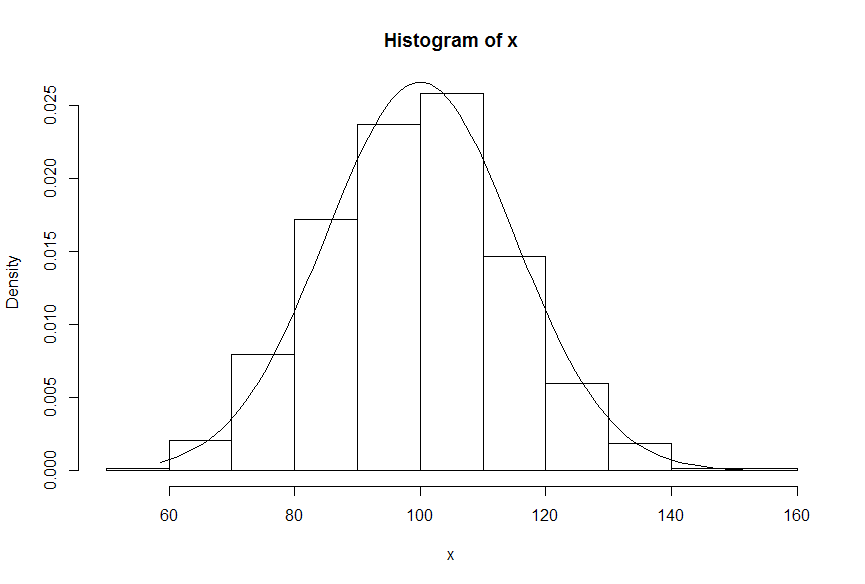
\includegraphics[width=\linewidth]{mal-01.png}
	\end{figure}

	\item Гама-розподіл. Знайдемо $P \{ X > 1 \}$, де $X$ має гама-розподіл з параметрами $ a = 2$, $\lambda = 3$.
	\begin{verbatim}
	> 1 - pgamma(1, 2, 3)
	[1] 0.1991483
	\end{verbatim}

	\item Розподіл $\chi^2$. Знайдемо $P \{ 40 \le \chi^2 \le 50 \}$, де $\chi^2$ розподілена з \verb|65| степенями свободи.
	\begin{verbatim}
	> pchisq(50, 65) - pchisq(40, 65)
	[1] 0.07861696
	\end{verbatim}

	\item Розподіл Стьюдента. Знайдемо значення щільності розподілу Стьюдента з \verb|2| степенями свободи в точці \verb|0.8|.
	\begin{verbatim}
	> pt(0.8, 1)
	[1] 0.7147767
	\end{verbatim}
	Тут другий параметр обчислений за формулою = кількість степенів свободи $-1 = 2 - 1 = 1$.

	\item Розподіл Фішера. Знайдемо $c$, $d$ зі співвідношень $P\{ X < c\} = 0.95$ та $P \{ X < d\} = 0.05$, де $X$ має розподіл Фішера зі степенями свободи \verb|5|, \verb|10|.
	\begin{verbatim}
	> c <- qf(0.95, 5, 10)
	> c
	[1] 3.325835
	> d <- qf(0.05, 5, 10)
	> d
	[1] 0.2111904
	\end{verbatim}
\end{enumerate}

\section{Графічний аналіз}

В файлі \verb|Cancer.txt| наводяться дані по кількості викурених цигарок на душу населення в 43 регіонах Америки та округу Колумбія за 1960 рік, а також дані по кількості смертей від різних форм раку на 100 000 душ населення. Обсяг вибірки $n = 44$. Назви змінних:

\begin{enumerate}
	\item \verb|CIG| = Кількість викурених цигарок (умовних упаковок на душу населення).
	\item \verb|BLAD| = Кількість смертей на 100 тис. населення від раку сечового міхура
	\item \verb|LUNG| = Кількість смертей на 100 тис. населення від раку легенів.
	\item \verb|KID| = Кількість смертей на 100 тис. населення від раку нирки.
	\item \verb|LEUK| = Кількість смертей на 100 тис. населення від лейкемії.
\end{enumerate}

\begin{enumerate}
	\item Читаємо дані з файлу у фрейм \verb|da|.
	\begin{verbatim}
	> da <- read.table(file.choose(), header = TRUE)
	\end{verbatim}

	\item Побудуємо гістограму для змінної \verb|CIG|. Розбиття на часткові інтервали обирається за замовчанням.

	\begin{verbatim}
	> attach(da)
	> hist(CIG)
	\end{verbatim}

	\begin{figure}[H]
		\centering
		\includegraphics{mal-02.png}
	\end{figure}
	
	\item Якщо ми хочемо самотужки розбити на часткові інтервали наші дані, слід скористатись опцією \verb|breaks|. Часткові інтервали довжини \verb|3|, від \verb|0| до \verb|50|. \verb|Xlab| використовується для надпису на осі $ОХ$.

	\begin{verbatim}
	> bin <- seq(0, 50, 3)
	> hist(CIG, breaks = bin, xlab = "Cigarettes", right = FALSE)
	\end{verbatim}

	\begin{figure}[H]
		\centering
		\includegraphics{mal-03.png}
	\end{figure}

	\item Для побудови вусатої коробочки (англ. boxplot) можна скористатись оператором

	\begin{verbatim}
	> boxplot(CIG)
	\end{verbatim}

	\begin{figure}[H]
		\centering
		\includegraphics{mal-04.png}
	\end{figure}

	В пакеті R вусата коробочка має традиційну структуру. Середня риска коробочки відмічає вибіркову медіану. Прямокутник відмічає нижній ($H_l$) і верхній ($H_u$) квартилі. Тобто, $H_l$ -- вибірковий квантиль рівня $1/4$; $H_u$ -- вибірковий квантиль рівня $3/4$. Позначимо ширину прямокутника $H = H_u - H_l$. Тоді відстань від прямокутника до верхнього вуса коробочки становить $1.5Н$; в нижній частині коробочки так само $1.5Н$.

	\item Побудуємо 4 коробочки на одному графіку: \verb|BLAD|, \verb|LUNG|, \verb|KID|, \verb|LEUK|.

	\begin{verbatim}
	> boxplot(BLAD, LUNG, KID, LEUK, horizontal = TRUE, 
		col = c(13, 4, 1, 2), names 
		= c("BLAD", "LUNG", "KID", "LEUK"))
	\end{verbatim}

	\begin{figure}[H]
		\centering
		\includegraphics{mal-05.png}
	\end{figure}

	Опція \verb|horizontal = TRUE| задає горизонтальне положення вусатих коробочок, опція \verb|col| описує кольори, в які вони пофарбовані, \verb|names| друкує надписи до коробочок.

	\item Побудувати Q-Q (quantile-quantile) діаграму на порівняння з нормальним розподілом можна наступним чином

	\begin{verbatim}
	> qqnorm(CIG)
	> qqline(CIG)
	\end{verbatim}
	
	\begin{figure}[H]
		\centering
		\includegraphics{mal-06.png}
	\end{figure}
	
	Тепер побудуємо Q-Q-діаграму на порівняння змінної \verb|CIG| з розподілом $\chi^2$ з п’ятьма степенями свободи. Як ми знаємо, обсяг вибірки $= 44$. Опція \verb|ppoints| задає послідовність чисел $\frac{i - 1/2}{n}$, в даному випадку $n = 44$.
	
	\begin{verbatim}
	> qqplot(CIG, qchisq(ppoints(44), df = 5))
	\end{verbatim}
	
	\begin{figure}[H]
		\centering
		\includegraphics{mal-07.png}
	\end{figure}
	
	\item Побудувати P-P (probability-probability plot) діаграму на порівняння з нормальним розподілом можна наступним чином. Як відомо, абсциса точки на p-p-діаграмі є емпірична функція розподілу, куди замість аргументу підставляємо дані з вибірки, ордината -- теоретична функція розподілу, куди так само замість аргументу підставляємо дані з вибірки. Емпіричну функцію розподілу можна побудувати за допомогою функції \verb|ecdf()|. В наступному прикладі ми генеруємо вибірку зі стандартним нормальним розподілом і будуємо для неї p-p-діаграму на порівняння з тим самим нормальним розподілом.
	
	\begin{verbatim}
	> x <- rnorm(100, 0, 1)
	> plot(ecdf(x), pnorm(x, mean(x), sd(x)))
	\end{verbatim}
	
	Друга з команд проводить пряму.
	
	\begin{figure}[H]
		\centering
		\includegraphics{mal-08.png}
	\end{figure}
	
	\item Побудуємо матричну діаграму всіх змінних, розміщених в \verb|Cancer.txt|, тобто, тепер в фреймі \verb|da|.
	
	\begin{verbatim}
	> pairs(da)
	\end{verbatim}
	
	\begin{figure}[H]
		\centering
		\includegraphics{mal-09.png}
	\end{figure}
	
	Схоже, що змінні \verb|BLAD| та \verb|LUNG| залежні лінійно від \verb|CIG|, а от \verb|KID| та \verb|LEUK| -- не дуже.
\end{enumerate}

\end{document}